\begin{frame}{Problem: OverFitting in a Neural Network}
	\begin{itemize}
		\item Why does overfitting happen in a neural network?
		\begin{itemize}
			\item There are \tc{keywords}{Too many free parameters}.
		\end{itemize}
	\end{itemize}
    \begin{figure}[H]
        \centering
        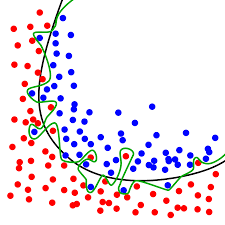
\includegraphics[width=0.4\textwidth]{Figs/section_4/overfitting.png}
        \caption{OverFitting in a neural network. \href{https://en.wikipedia.org/wiki/Overfitting}{source}}
    \end{figure}
\end{frame}

\begin{frame}{Solution 1: L1/L2 Regularization}
    \begin{itemize}
        \item It is like a linear regression regularizer.
        \item Sum the regularizer term for every \tc{keywords}{layer weight}!
    \end{itemize}
    \vspace{0.2\textheight}
    \begin{equation*}
        \mathlarger{\mathlarger{\mathlarger{
        L = \frac{1}{N} \sum_{i=1}^{N} L(\phi(x_i), y_i) + \lambda \sum_{i,j,k} R(W_{j,k}^{(i)})
        }}}
    \end{equation*}
\end{frame}
\begin{frame}{Solution 1: L1/L2 Regularization}
    \begin{itemize}
        \item L1/L2 regularizer functions (review)
    \end{itemize}
	\begin{columns}
		\begin{column}[c]{0.5\textwidth}
			\centering
			\begin{equation*}
				\centering
				\mathlarger{\mathlarger{
							L1: R(w) = \vert w\vert
				}}
			\end{equation*}
			\begin{equation*}
				\centering
				\mathlarger{\mathlarger{
							L2: R(w) = w^2
				}}
			\end{equation*}
		\end{column}
		\begin{column}[c]{0.5\textwidth}
			\begin{figure}[H]
				\centering
				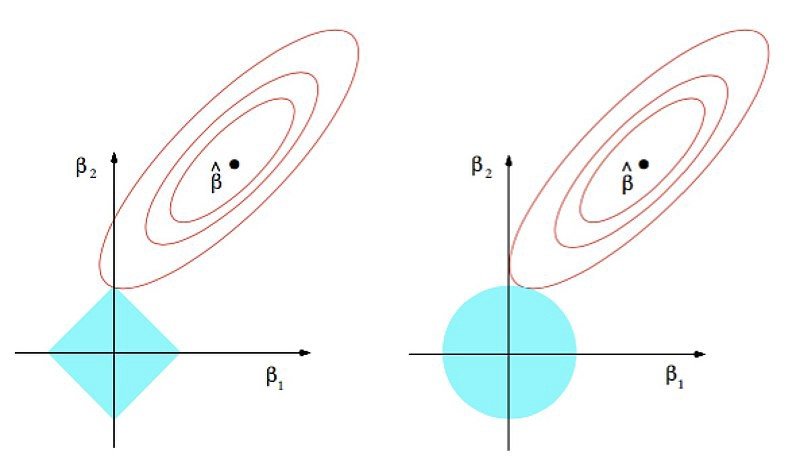
\includegraphics[width=\textwidth]{Figs/section_4/l1l2_reg.jpeg}
				\caption{L1/L2 regularizers' solution diagram \href{https://towardsdatascience.com/understanding-l1-and-l2-regularization-93918a5ac8d0}{source}}
			\end{figure}
		\end{column}
	\end{columns}
    
    \begin{itemize}
        \item You can also combine the two different regularizers (Elastic Net).
    \end{itemize}
    \begin{equation*}
        \mathlarger{\mathlarger{
        R(w) = \beta w^2 + \vert w\vert
        }}
    \end{equation*}
\end{frame}

\begin{frame}{Solution 2: Early Stopping}
    \begin{itemize}
        \item Stop the training procedure when the validation error is \tc{keywords}{minimum}.
    \end{itemize}
    \begin{figure}
	\centering
	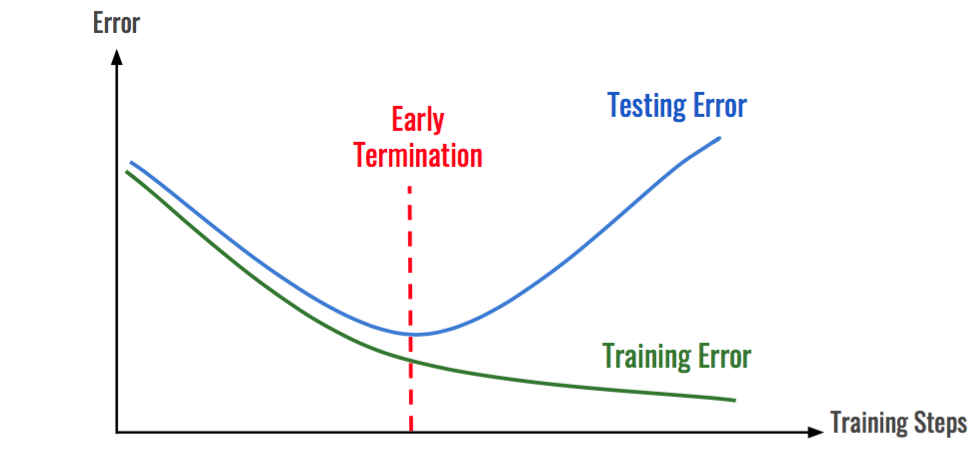
\includegraphics[width=0.8\textwidth]{Figs/Early Stopping.png}
	\caption{Early-Stopping diagram. \href{https://medium.com/analytics-v7idhya/early-stopping-with-pytorch-to-restrain-your-model-from-overfitting-dce6de4081c5}{source}}
    \end{figure}
\end{frame}

\begin{frame}{Solution 3: Dropout}
	\begin{block}{Training}
		\begin{itemize}
			\item at each iteration, every neuron has a probability $P$ of being dropped out
			\begin{itemize}
				\item meaning it will be ignored
			\end{itemize}
			\item $P :=$ dropout rate
		\end{itemize}
		
		\begin{figure}[H]
			\centering
			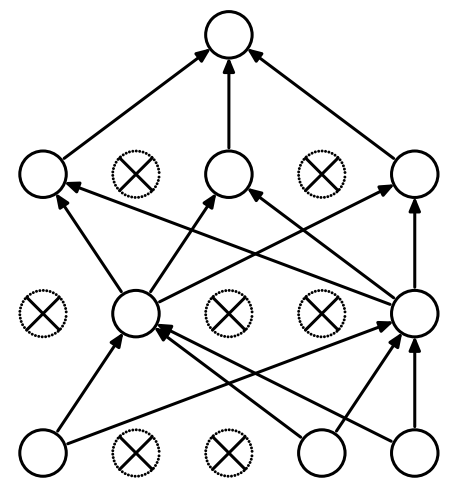
\includegraphics[height=0.4\textheight]{Figs/Dropout-after.png}
			\caption{Behavior of dropout at training time. \href{https://www.cs.toronto.edu/~hinton/absps/JMLRdropout.pdf}{Source}}
		\end{figure}
	\end{block}
\end{frame}
\begin{frame}{Solution 3: Dropout}
	\begin{block}{Testing}
		\begin{itemize}
			\item at each iteration, on average, 1-P percent of Neurons are active
			\begin{itemize}
				\item less neurons results in bigger weights
			\end{itemize}
			\item we need to normalize weights by 1-P
		\end{itemize}
		
		\begin{figure}[H]
			\centering
			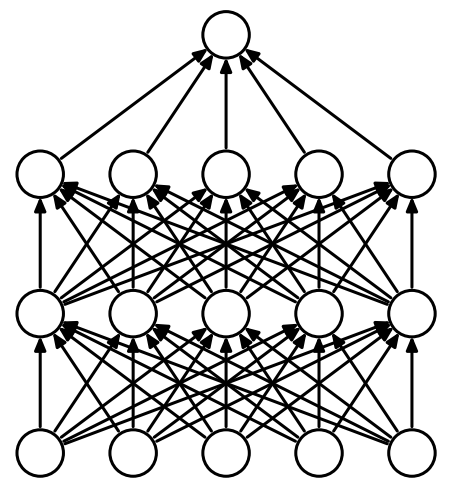
\includegraphics[height=0.4\textheight]{Figs/Dropout-before.png}
			\caption{Behavior of dropout at testing time. \href{https://www.cs.toronto.edu/~hinton/absps/JMLRdropout.pdf}{Source}}
		\end{figure}
	\end{block}
\end{frame}
\begin{frame}{Solution 3: Dropout}
	\begin{block}{Performance}
		\begin{itemize}
			\item the dependence between different neuron decreases
			\begin{itemize}
				\item neurons get more generalized
			\end{itemize}
		\end{itemize}
		
		\begin{figure}[H]
			\centering
			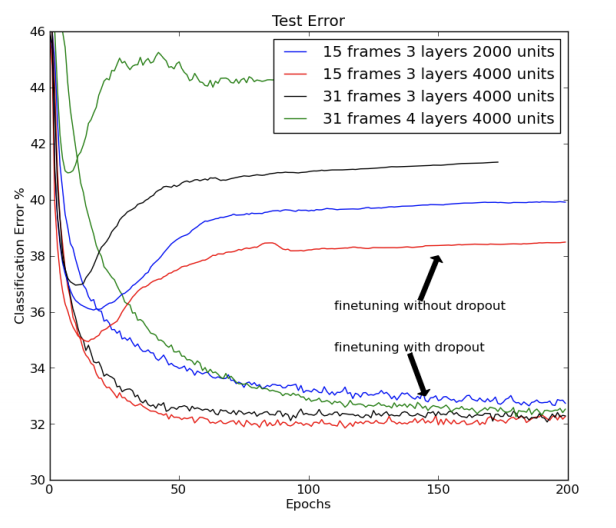
\includegraphics[height=0.4\textheight]{Figs/section_4/dropout_performance.png}
			\caption{the effect of dropout layer. as you see, the total error is reduced by a considerable amount. \href{https://towardsdatascience.com/understanding-and-implementing-dropout-in-tensorflow-and-keras-a8a3a02c1bfa}{Source}}
		\end{figure}
	\end{block}
\end{frame}
\begin{frame}{Solution 3: Dropout}
	\begin{block}{Practice tips}
		\begin{itemize}
			\item you can tweak dropout rate if you still see overfitting issues
			\begin{itemize}
				\item still overfitting -> increase dropout rate
				\item underfitting -> decrease dropout rate
			\end{itemize}
			\item layersize $\sim$ dropout rate
			\item usually in practice, people will use dropout after the last hidden layer
		\end{itemize}
	\end{block}
\end{frame}



\begin{frame}{Problem: Vanishing/Exploding Gradients}
	// Todo
    \begin{itemize}
    	\item beginning of learning -> He/ELU
    	\item during learning -> still exists
    \end{itemize}
    
    \begin{figure}[H]
    	\centering
    	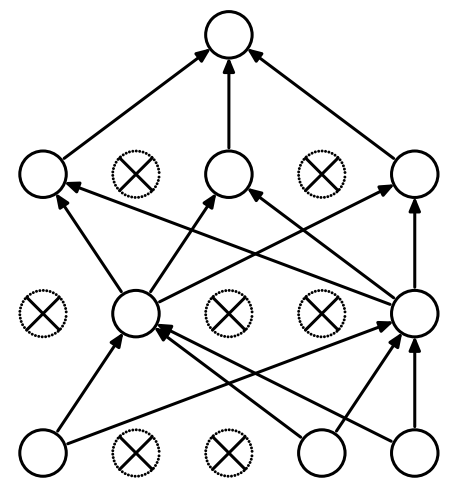
\includegraphics[height=0.4\textheight]{Figs/Dropout-after.png}
    	\caption{Behavior of dropout at training time. \href{https://www.cs.toronto.edu/~hinton/absps/JMLRdropout.pdf}{Source}}
    \end{figure}
\end{frame}

\begin{frame}{Solution: Batch Norm Layer}
	\begin{itemize}
		\item It is used for \tc{keywords}{normalizing} the data.
	\end{itemize}
	\begin{figure}[H]
		\centering
		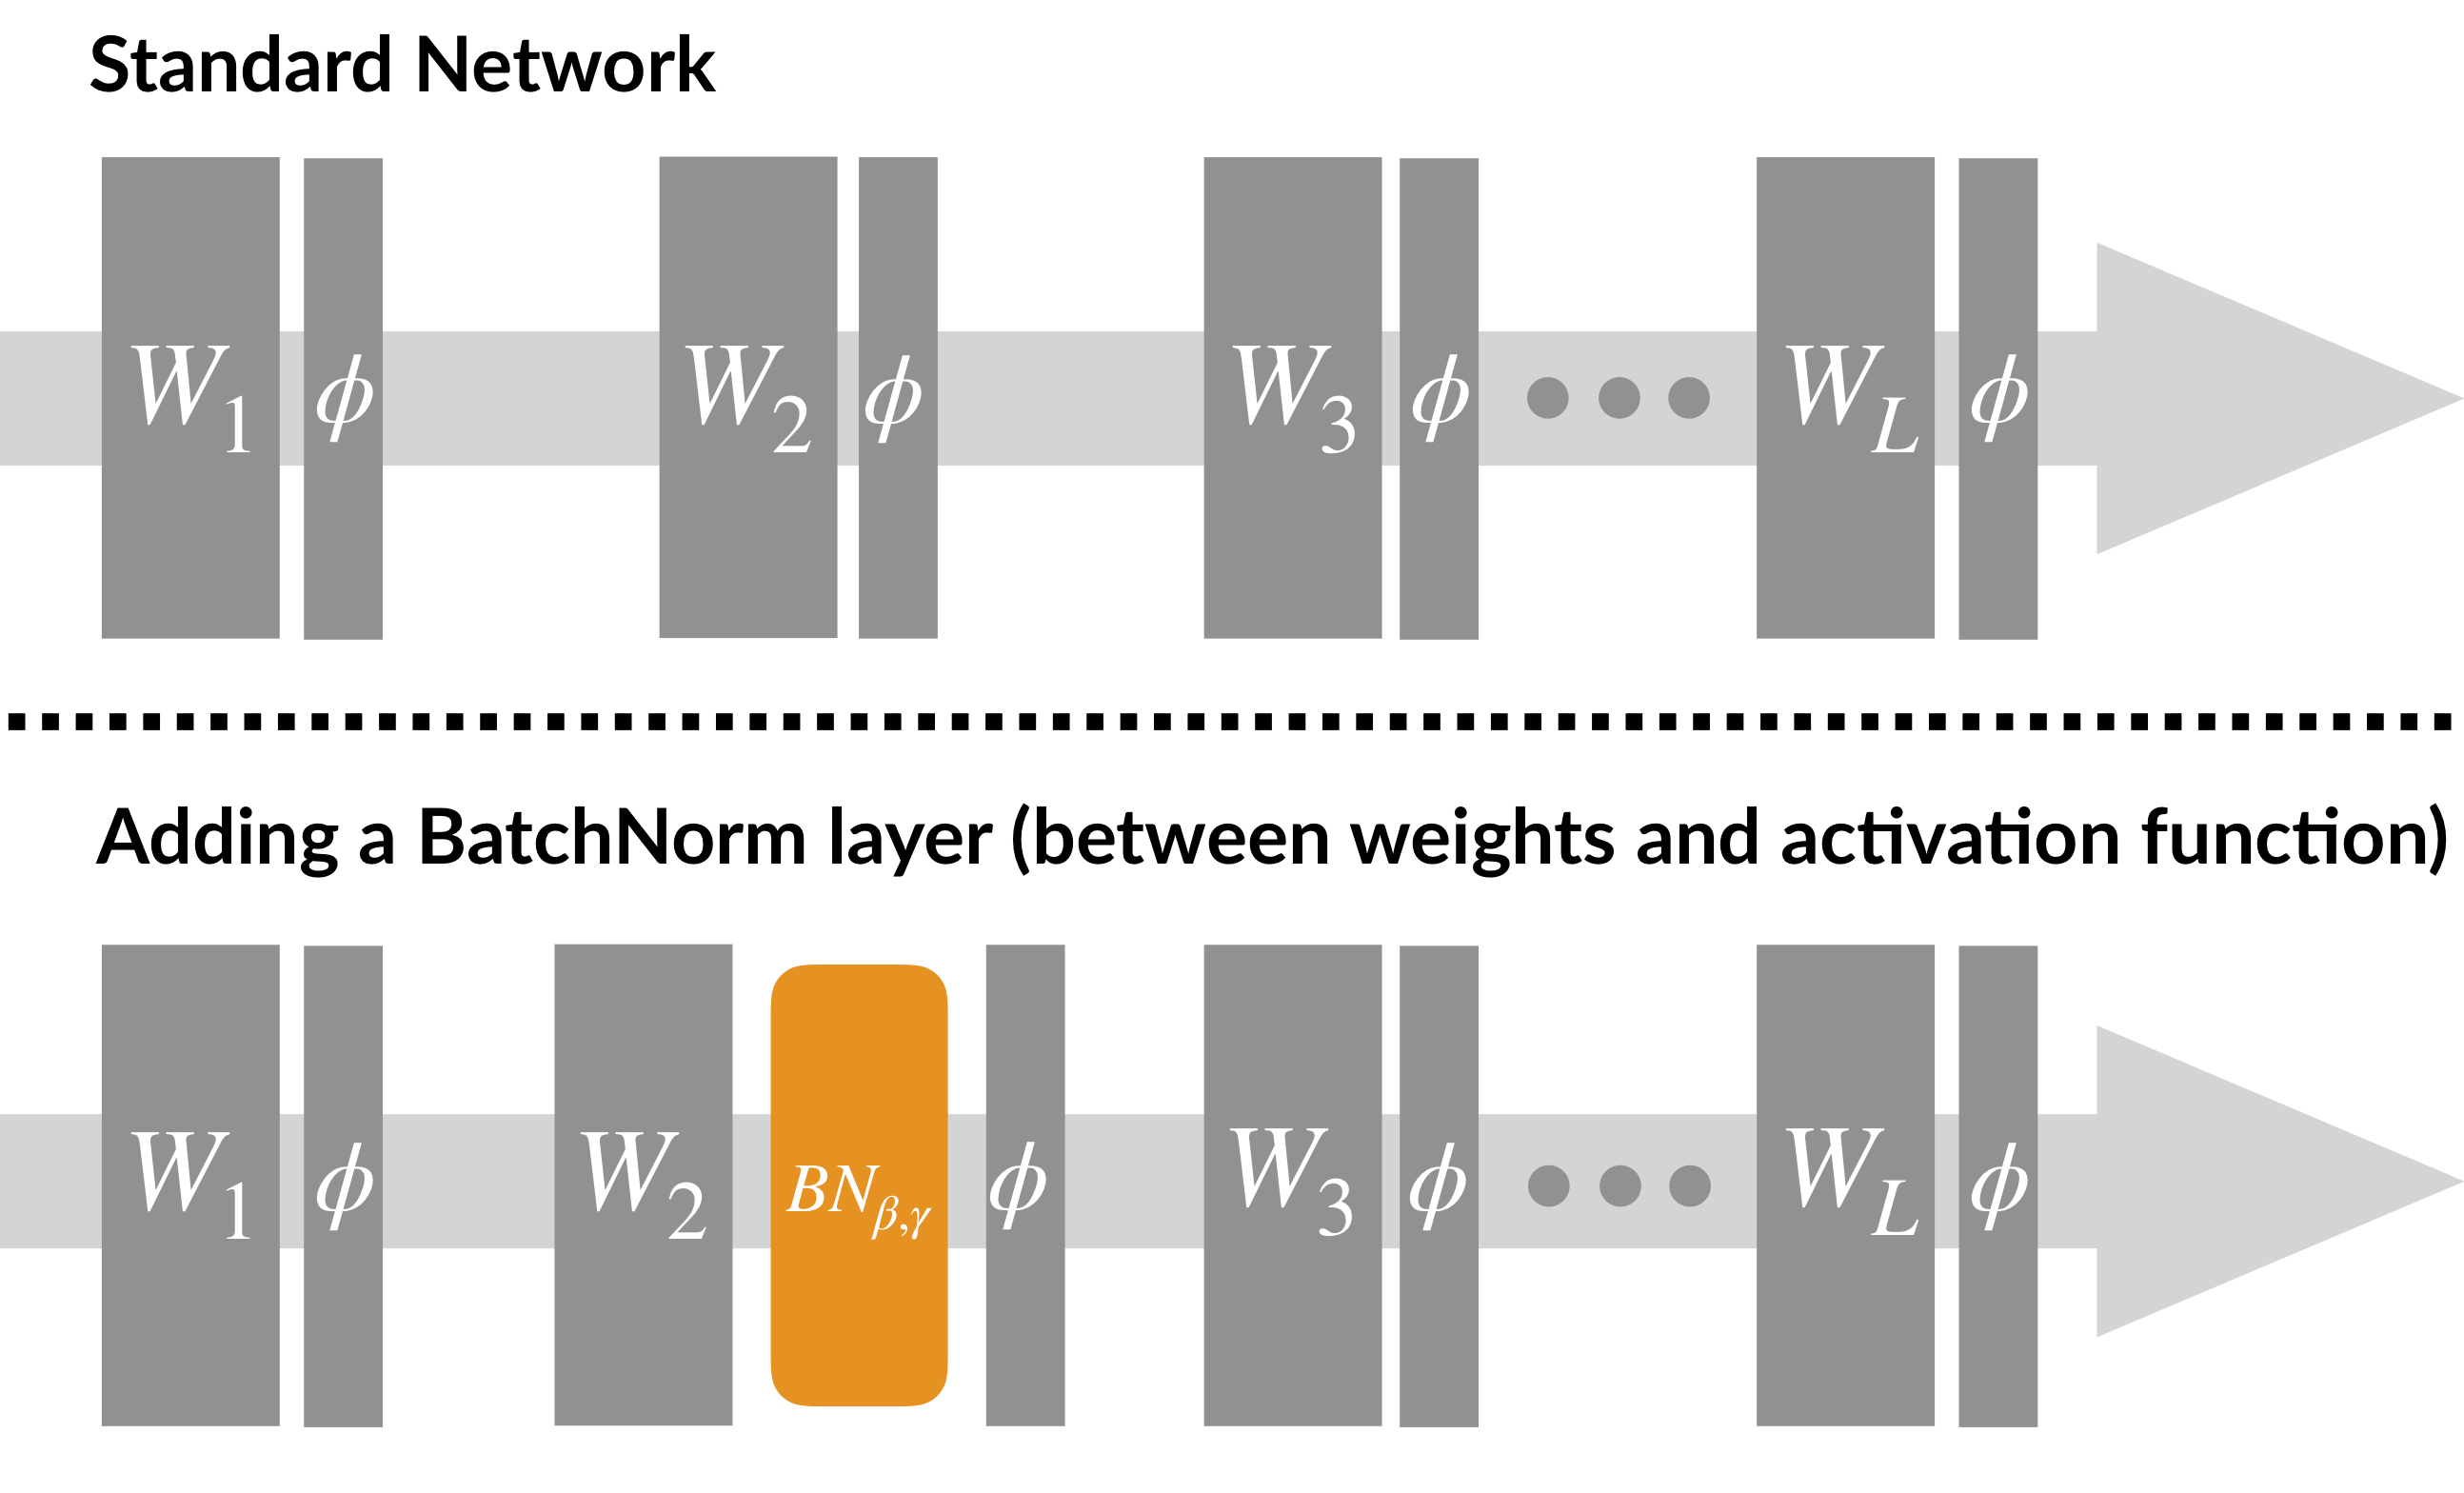
\includegraphics[width=0.75\textwidth]{Figs/section_4/batchnorm_2.jpg}
		\caption{The suggested place to put a BatchNorm layer. \href{https://gradientscience.org/batchnorm/}{source}}
	\end{figure}
\end{frame}
\begin{frame}{Solution: Batch Norm Layer}
	\begin{block}{Training}
		\begin{itemize}
			\item First, it zero-centers and normalizes the batch.
		\end{itemize}
		\begin{equation*}
			\mathlarger{
				\mu_B := \frac{1}{N_B} \sum{x_B^{(i)}}
			}
		\end{equation*}
		\begin{equation*}
			\mathlarger{
				\sigma_B^2 := \frac{1}{N_B} \sum{(x_B^{(i)} - \mu_B)^2}
			}
		\end{equation*}
		\begin{equation*}
			\mathlarger{
				\hat{x_B}^{(i)} = \frac{x_B^{(i)} - \mu_B}{\sqrt{\sigma^2_B + \epsilon}}
			}
		\end{equation*}
		\begin{itemize}
			\item Then, scales and shifts the batch with two learnable parameters $\gamma, \beta$.
		\end{itemize}
		\begin{equation*}
			\mathlarger{
				y_B^{(i)} = \gamma \hat{x_B}^{(i)} + \beta	
			}
		\end{equation*}
	\end{block}
\end{frame}
\begin{frame}{Solution: Batch Norm Layer}
	\begin{block}{Testing}
		\begin{itemize}
			\item To zero-center and normalize the input, we need average and variance of the whole data.
			\item Those parameters can be acquired during the training.
			\item Therefore we need two more trainable parameters.
		\end{itemize}
		\vspace{0.1\textheight}
			\begin{equation*}
				\mathlarger{
					\mu_D := \frac{1}{N} \sum{x^{(i)}}
				}
			\end{equation*}
			\begin{equation*}
				\mathlarger{
					\sigma_D^2 := \frac{1}{N} \sum{(x^{(i)} - \mu)^2}
				}
			\end{equation*}
	\end{block}
\end{frame}
\begin{frame}{Solution: Batch Norm Layer}
	\begin{block}{Performance}
		\begin{itemize}
			\item Normalizing the data improves the convergence speed by a considerable amount.
		\end{itemize}
		\begin{figure}[H]
			\centering
			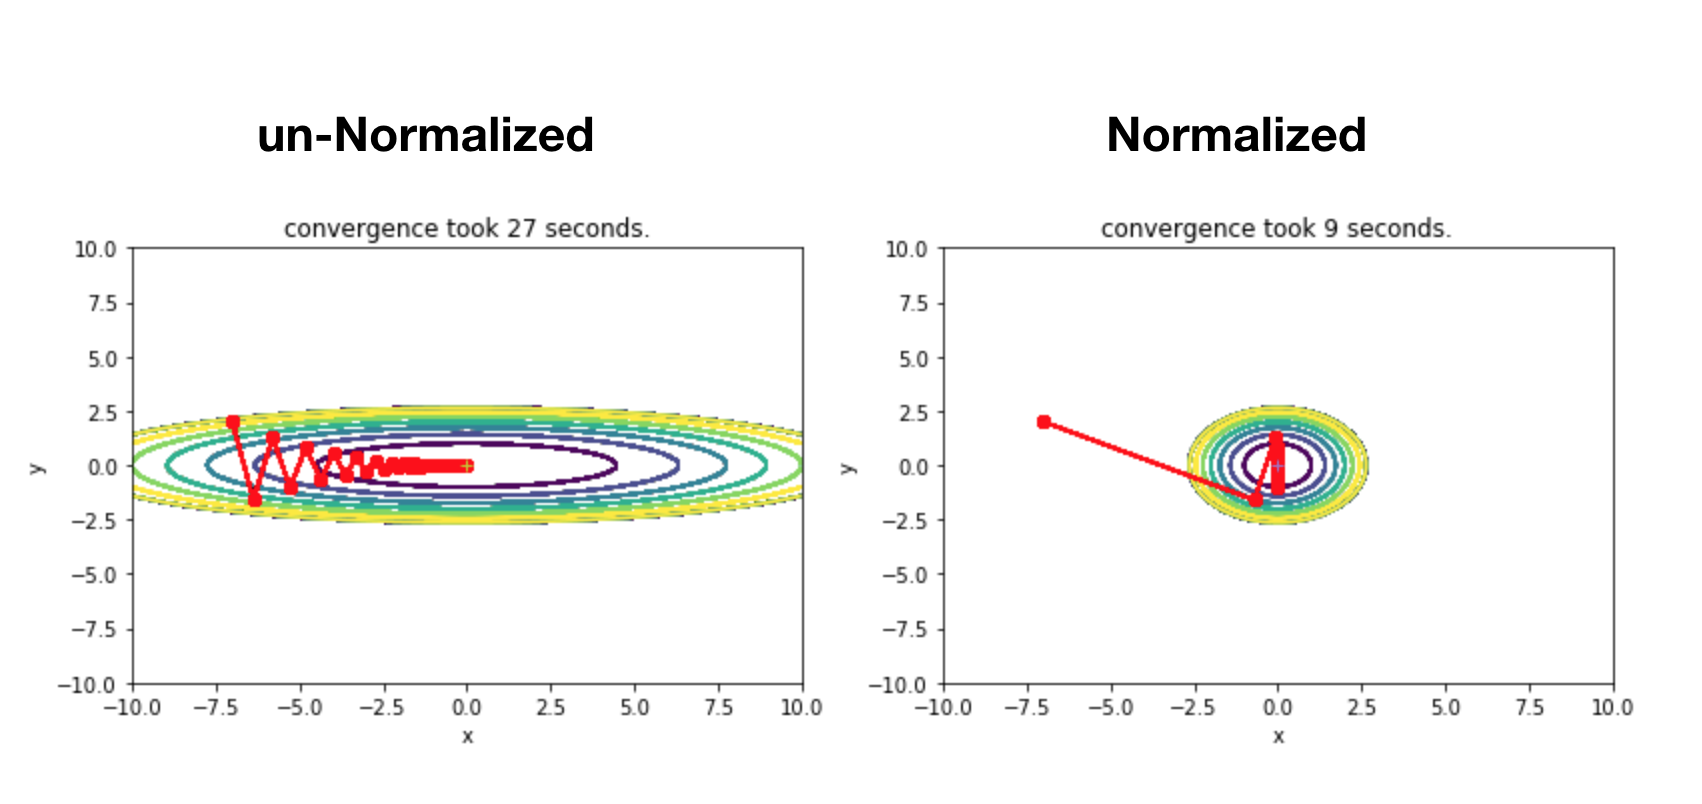
\includegraphics[width=0.8\textwidth]{Figs/section_4/batchnorm_3.png}
			\caption{BatchNorm performance. Convergence speed is increased by 200\%.  \href{https://jsideas.net/batch_normalization/}{source}}
		\end{figure}
	\end{block}
\end{frame}
\begin{frame}{Solution: Batch Norm Layer}
	\begin{block}{Pros}
		\begin{itemize}
			\item Vanishing/Exploding gradient problem is reduced by a considerable amount.
			\medskip
%			\begin{itemize}
				\item You can use even saturating activation functions.
				\medskip
				\item The network is much less sensitive to initial weight.
				\medskip
				\item We're able to use larger learning rates, which speeds up the training.
%			\end{itemize}
			\medskip
			\item It also acts as a regularizer.
			\medskip
			\begin{itemize}
				\item There is no need for other regularizer techniques.
			\end{itemize}
		\end{itemize}
	\end{block}
\end{frame}
\begin{frame}{Solution: Batch Norm Layer}
	\begin{block}{Cons}
		\begin{itemize}
			\item It increases model parameters and prediction latency.
			\begin{itemize}
				\item After the training procedure, we can mix the BatchNorm layer with its previous layer to hold the prediction latency.
			\end{itemize}
		\end{itemize}
		\begin{columns}
			\begin{column}[c]{0.45\textwidth}
				\centering
				\begin{equation*}
					\mathlarger{x'^{(i)} = W x^{(i)} + b}
				\end{equation*}
				\begin{equation*}
					\mathlarger{y^{(i)} = \frac{x'^{(i)} - \mu}{\sqrt{\sigma^2 + \epsilon}} + \beta}
				\end{equation*}
			\end{column}
			\begin{column}[c]{0.1\textwidth}
				\centering
				\begin{equation*}
					\mathlarger{\mathlarger{
					\Rightarrow
				}}
				\end{equation*}
			\end{column}
			\begin{column}[c]{0.45\textwidth}
				\centering
				\begin{equation*}
					\mathlarger{y^{(i)} = W' x^{(i)} + b'}
				\end{equation*}
				\begin{equation*}
					\mathlarger{
						W' := \frac{1}{\sqrt{\sigma^2 + \epsilon}} W	
					}
				\end{equation*}
				\begin{equation*}
					\mathlarger{
						b' := \beta + \frac{b- \mu}{\sqrt{\sigma^2 + \epsilon}}	
					}
				\end{equation*}
			\end{column}
		\end{columns}
	\end{block}
\end{frame}